\subsection{Selección de Ventana}
\label{sec:window_selection}

En esta sección discutiremos los parámetros \emph{tamaño de ventana} o \emph{frame size} y el \emph{frame step}. En el trabajo \cite{KOU2008.2} se menciona una elección de \emph{frame step} y \emph{frame length} de 10s y 20s respectivamente. En el caso de nuestro corpus, queremos buscar los parámetros que mejor se ajustan a éste, manteniendo la superposición del 50\% entre ventanas sucesivas.

¿Qué queremos optimizar? El criterio que elegimos para esto es encontrar un balance entre una ventana no tan grande (para no suavizar en exceso la curva) y que nos reduzca considerablemente la cantidad de indefiniciones; es decir, aquellas ventanas que tomamos en un hablante que no tienen ninguna participación medible de su parte. Para ver esto, graficamos la cantidad de indefiniciones en función del step tomado, para ver qué forma tenían estas curvas. En la Figura \ref{fig:window_selection_session} podemos ver las indefiniciones en función de los steps para una sesión del corpus. Cada tarea tiene su propia curva, y además graficamos el promedio de todas ellas.

\begin{figure}
\centering
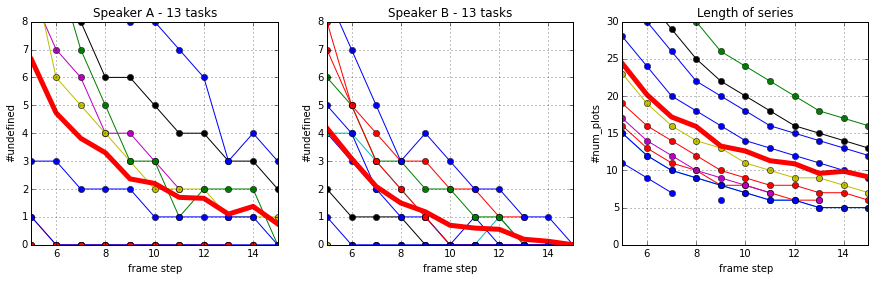
\includegraphics[width=15cm]{images/window_selection_for_session.png}
\caption{Cantidad de puntos indefinidos en función del step para una sesión en particular, tanto para un interlocutor como para el otro. En rojo se grafica la curva de los promedios}
\label{fig:window_selection_session}
\end{figure}

Finalmente, para tener una visión general de lo que ocurría, graficamos una curva promedio de todas las sesiones, que se ilustra en la Figura \ref{fig:window_selection_average}. Sobre esta curva aplicamos el ``método del codo'' para ver si podemos encontrar el valor en el cual la pendiente de las indefiniciones se estanca. Si bien es poco preciso hacer esto, puede observarse que hasta 8-10 segundos hay un fuerte descenso de las indefiniciones, que luego se atenúa. Dado que en general tenemos tareas cortas, preferimos tomar 8 segundos como step, y por ende 16 segundos como largo de ventana.

\begin{figure}[bh!]
\centering
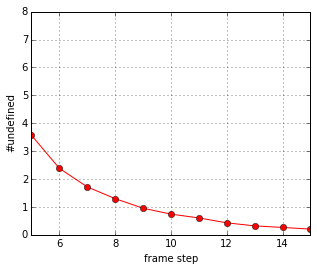
\includegraphics[scale=0.75]{images/window_selection.png}
\caption{Promedio de cantidad de puntos indefinidos en función del step}
\label{fig:window_selection_average}
\end{figure}


